\documentclass[a4paper, 11pt]{article}
\usepackage[top=30mm, bottom=35mm, left=25mm, right=25mm]{geometry}
\usepackage{fancyhdr, graphicx}
\usepackage{amsmath}
\usepackage{amsthm}
\usepackage{fancyvrb}
\usepackage[pagebackref=false,colorlinks,linkcolor=blue,citecolor=blue]{hyperref}
\usepackage{longtable}
\usepackage{enumitem}
\usepackage[extrafootnotefeatures, localise]{xepersian}
\settextfont[Scale=1]{XB Niloofar}
\setlatintextfont[Scale=0.9]{XB Niloofar}
\linespread{1.6}
\newcommand{\مل}{\متن‌لاتین}
\newcommand{\tlr}[1]{\text{\lr{#1}}}
\newcommand{\ورب}[1]{\lr{\Verb!#1!}}
\usepackage{comment}
\usepackage{titling}
\pagestyle{fancy}
\fancyhead[L]{}
\fancyhead[R]{\it{\thetitle}}
\setlength{\headheight}{27pt}
\fancypagestyle{plain}
{
	\fancyhead[R]{}
	\fancyhead[C]{\hspace{-0.3cm}به نام خدا}
	\fancyhead[L]{}
	\renewcommand{\headrulewidth}{0pt}
}

\عنوان{مستندات بلوک شبیه‌ساز شبکه سیمولینک}
\نویسنده{محمد فرزان}
\تاریخ{نسخهٔ ۱ $\vert$ \امروز}
\شروع{document}
{\let\newpage\relax\maketitle}
\قسمت*{فهرست تغییرات}
\ورودی{changelog}
\فهرست‌مطالب
\صفحه‌جدید
\قسمت{مقدمه}
بلوک شبکهٔ سیمولینک برای شبیه‌سازی اثرات شبکهٔ اینترنت به کار می‌رود. در حال حاضر این بلوک قابلیت‌های زیر را دارد:
\شروع{فقرات}
\فقره نمونه‌برداری از ورودی پیوسته با نرخ قابل تنظیم
\فقره شبیه‌سازی تاخیر\پانویس{Latency} با مقدار ثابت یا متغیر با توزیع گوسی
\فقره شبیه‌سازی جابجایی ترتیب بستک‌ها\پانویس{Packet reordering} ناشی از تاخیر متغیر
\فقره شبیه‌سازی از دست رفتن بستک‌ها\پانویس{Packet loss} با دو مدل تصادفی مستقل و زنجیرهٔ مارکوف\پانویس{Markov chain}
\پایان{فقرات}

\قسمت{تعاریف}
در سراسر این متن، تعاریف زیر مورد استفاده قرار می‌گیرند:
\شروع{فقرات}
\فقره[] \متن‌سیاه{تاخیر:} به فاصله زمانی میان ارسال اولین بیت یک بستک از سیستم مبدأ تا زمان دریافت آخرین بیت همان بستک در سیستم مقصد گفته می‌شود. در صورتی که بستک در مقصد دریافت نشود مقدار این کمیت تعریف نشده است، اما در کاربردهای غیر رسمی ممکن است با بی‌نهایت نمایش داده شود. \مرجع{rfc7679}
\فقره[] \متن‌سیاه{اتلاف بستک:} یک مقدار عددی برابر با صفر یا یک است. مقدار اتلاف صفر به معنای رسیدن بستک به مقصد و مقدار یک به معنای نرسیدن آن می‌باشد. زمان نسبت داده شده به کمیت برابر با زمانی است که فرستنده اولین بیت را ارسال می‌کند. \مرجع{rfc7680}
\فقره[] \متن‌سیاه{تغییرات تاخیر:} به اختلاف مقدار تاخیر دو بستک گفته می‌شود. \مرجع{rfc3393}
\فقره[] \متن‌سیاه{تغییر ترتیب بستک:} مقدار تغییر ترتیب برای بستک با شماره ترتیبی\پانویس{Sequence number} $s$ صحیح است اگر و فقط اگر هنگام رسیدن بستک به مقصد داشته باشیم $s<\tlr{NextExp}$؛ جایی که \مل{NextExp} برابر با مقدار شماره ترتیبی مورد انتظار بستک دریافتی در مقصد است. \مرجع{rfc4737}
\پایان{فقرات}

\قسمت{راهنمای نصب}
\شروع{شمارش}
\فقره آخرین نسخهٔ پکیج را از 
\href{https://github.com/m2-farzan/simulink-network-emulator/releases/latest/download/IDAS-Network-Emulator.mltbx}%
{این لینک} بارگیری کنید.
\فقره نرم‌افزار متلب را باز نموده و از پنل مرورگر فایل آن، به پوشهٔ محل دانلود بروید.
\فقره در پنل مرورگر فایل متلب، روی \ورب{IDAS-Network-Emulator.mltbx} جفت کلیک کنید.
\فقره در پنجرهٔ باز شده روی گزینهٔ \مل{Install} کلیک کنید.
\فقره اکنون کتابخانه نصب شده است. برای تایید نصب، سیمولینک را باز کرده و وارد \مل{Library Browser} شوید. اگر این پنجره از قبل باز است، کلید \مل{F5} را بزنید.
\فقره در صورت نصب صحیح باید در لیست تولباکس‌ها آیتم \مل{IDAS Network Emulator} اضافه شده باشد. (شکل زیر)
\پایان{شمارش}
\begin{figure}[h]
\centering
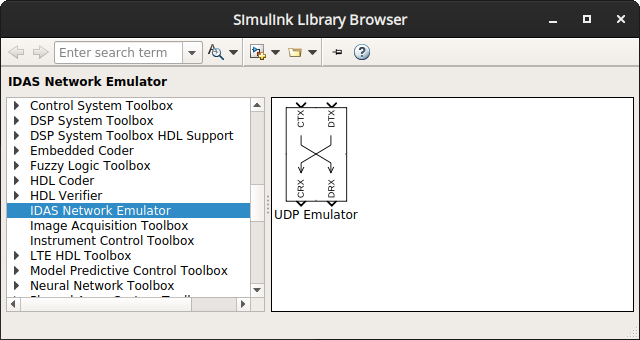
\includegraphics[width=12cm]{img/good-install}
\شرح{نصب موفق}
\برچسب{نصب موفق}
\end{figure}

\قسمت{راهنمای استفاده}
پیش از استفاده از بلوک \مل{UDP Emulator} به این نکته توجه کنید که حلگر سیمولینک باید در حالت گام-متغیر باشد. این حالت تنظیمات پیشفرض سیمولینک است و در صورتی که آن را تغییر نداده باشید، جای نگرانی وجود ندارد.
\شروع{شمارش}
\فقره بلوک \مل{UDP Emulator} را به درون مدل سیمولینک خود بکشید.
\فقره اتصالات لازم را انجام دهید. بلوک دو کانال دارد که یکی برای انتقال اطلاعات از ابر (C) به دستگاه (D) و دیگری برای بازگشت اطلاعات از دستگاه (D) به ابر (C) است. به طور دقیق، اتصالات به صورت زیر است:
\شروع{فقرات}
\فقره \متن‌سیاه{\ورب{CTX}}: داده‌ای که ابر به شبکه ارسال می‌کند.
\فقره \متن‌سیاه{\ورب{DRX}}: داده‌ای که دستگاه از شبکه دریافت می‌کند.
\فقره \متن‌سیاه{\ورب{DTX}}: داده‌ای که دستگاه به شبکه ارسال می‌کند.
\فقره \متن‌سیاه{\ورب{CRX}}: داده‌ای که ابر از شبکه دریافت می‌کند.
\پایان{فقرات}
پس از اتصال، مدل مانند شکل \رجوع{مدل} خواهد بود. دقت شود که لازم نیست که هر دو کانال متصل باشند؛ یعنی ارتباط می‌تواند یک طرفه باشد. همچنین در صورتی که لازم باشد به جای کمیت اسکالر، یک بردار در شبکه فرستاده شود، لازم است ابتدا با استفاده از بلوک \مل{Vector Concatenate} سیگنال‌ها به یک تک سیگنال برداری تبدیل شوند. این سیگنال می‌تواند به شبکه فرستاده شود و لازم است در طرف مقابل نیز سیگنال با استفاده از بلوک \مل{Submatrix} از حالت برداری خارج شود. در این رابطه یک مثال در پوشهٔ \مل{examples}، فایل \مل{VectorMode} وجود دارد.
\begin{figure}[h]
\centering
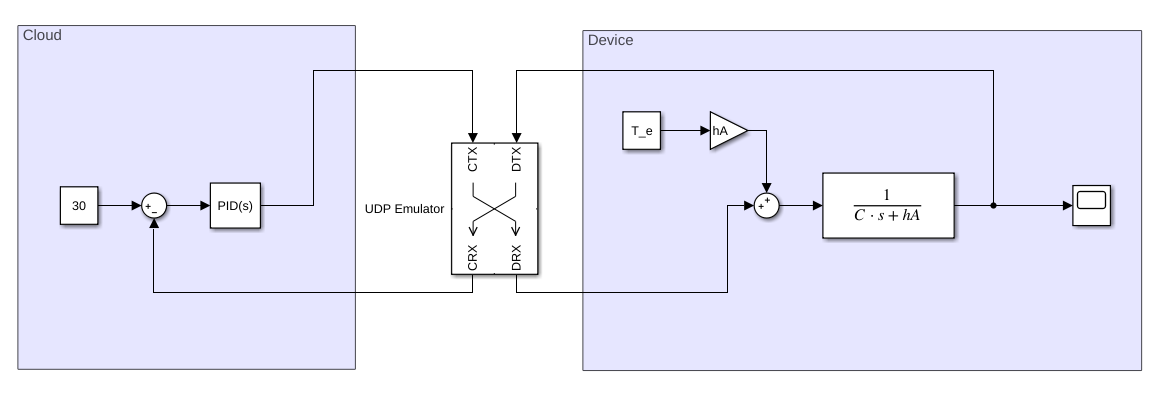
\includegraphics[width=16cm]{img/model.png}
\شرح{نحوهٔ اتصال صحیح شبکه (فایل این مدل در پوشهٔ \مل{examples} فایل \مل{RemotePidController} موجود است.)}
\برچسب{مدل}
\end{figure}
\فقره روی بلوک جفت کلیک کنید تا پنجرهٔ پارامترها باز شود (شکل \رجوع{پنجرهٔ پارامترها}). پارامترها را بر اساس جدول زیر تنظیم کنید.
\begin{figure}
\centering
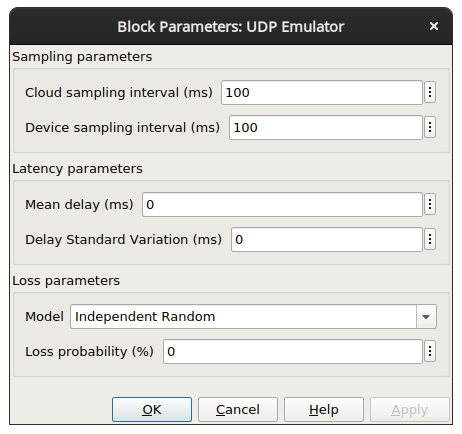
\includegraphics[width=8cm]{img/params-dialog.png}
\شرح{پنجرهٔ پارامترها}
\برچسب{پنجرهٔ پارامترها}
\end{figure}

\begin{longtable}{l|p{12cm}}
\multicolumn{1}{c|}{پارامتر} & \multicolumn{1}{c}{توضیحات} \\
\hline
\lr{Cloud sampling interval}&
مقدار این فیلد مشخص می‌کند که بستک‌های ارسالی از ابر به دستگاه هر چند میلی‌ثانیه ارسال شوند. در واقع این پارامتر، نرخ نمونه‌برداری سیگنال پیوستهٔ ورودی را مشخص می‌کند. در نسخه‌های آینده قابلیت تعریف ورودی گسسته نیز اضافه خواهد شد که در آن به محض تغییر سطح سیگنال ورودی، بستک تولید شده و ارسال می‌شود. \\ \hline
\lr{Device sampling interval} & مشابه پارامتر بالا، برای کانال دستگاه به ابر. \\ \hline
\lr{Mean delay} & مقدار متوسط تاخیر بستک‌ها را مشخص می‌کند. \\ \hline
\lr{Delay standard variation} & در صورتی که مقدار این پارامتر صفر باشد، تمام بستک ها با تاخیر برابر ارسال می‌شوند. در صورتی که مقدار این پارامتر مثبت باشد، تاخیر بستک‌ها توزیع نرمال خواهد داشت و مقدار این پارامتر برابر با انحراف معیار این توزیع خواهد بود. تاخیر هر بستک مستقل از بستک‌های دیگر است.
\\ \hline
\lr{Loss Model} & \setRTL مدل شبیه‌سازی از دست رفتن بستک‌ها که دو حالت دارد:
\شروع{فقرات}[rightmargin=0.5cm]
\فقره
\مل{Independent Random}: در این حالت، احتمال از دست رفتن هر بستک مستقل از بستک‌های دیگر است و پارامتر آن عبارت است از:
\شروع{فقرات} [rightmargin=1cm] \فقره \مل{Loss probability}: احتمال از دست رفتن بسته \پایان{فقرات}
\فقره
\lr{4-State Markov Chain}:
در این حالت، از دست رفتن بستک‌ها با یک مدل واقع گرایانه تر شبیه‌سازی می‌شود. در این مدل، شبکه دارای حالت\پانویس{State} است و از دست رفتن بستک‌ها به صورت رگباری\پانویس{Burst} رخ می‌دهد. پارامترهای این مدل به صورت زیر هستند:
\شروع{فقرات} [rightmargin=1cm] 
\فقره \مل{Loss probability}: مقدار کل احتمال از دست رفتن بسته
($P_\tlr{loss}$)
\فقره \مل{Mean burst length}: طول متوسط قطعی رگباری (بر حسب تعداد بستک)
($E(B)$)
\فقره \مل{Loss density within the burst}: احتمال از دست رفتن بسته در حالت قطعی رگباری
($\rho$)
\فقره \مل{Isolated loss probability}: احتمال از دست رفتن بسته در حالت غیر رگباری
($P_\tlr{isol}$)
\فقره \مل{Mean good burst length}: طول متوسط وصلی‌های رگباری میان یک قطعی رگباری (بر حسب تعداد بستک)
($E(GB)$)
\پایان{فقرات}
دقت شود که پارامترهای فوق باید شرایط زیر را ارضا کنند؛ در غیر این صورت پنجرهٔ پارامترها خطا می‌دهد:
\شروع{فقرات} [rightmargin=1cm] 
\item $E(B) \ge 1/\rho$
\item $P_\tlr{isol} \le P_\tlr{loss} < \rho$
\item $P_\tlr{loss} - P_\tlr{isol} \le E(B) (1-P_\tlr{isol})(\rho - P_\tlr{loss})$
\item $E(GB) \ge 1$
\item $E(GB) \ge (1-\rho)/\rho$
\item $P_\tlr{isol} \le 1/2$
\پایان{فقرات}
\پایان{فقرات}
\label{جدول پارامترها}
\end{longtable}
\پایان{شمارش}

\قسمت{مستندات پیاده‌سازی}
\زیرقسمت{مدل‌های انتخاب شده}
تاخیر بستک‌ها در قالب یک فرایند پواسون مدل شده است و بنابراین، فرض شده است که تاخیر هر بستک از سایر بستک‌ها مستقل است. این فرض اگرچه در بسیاری از موارد بیش از حد ساده است، اما در برخی مدل‌ها به اندازه کافی خوب عمل می‌کند \مرجع{Dahmouni2012}. مقدار تاخیر هر بستک به صورت تصادفی و با توزیع نرمال تولید می‌شود که مقدار متوسط و انحراف معیار توسط پارامترهای بلوک قابل تعریف هستند.

برای شبیه‌سازی اتلاف بستک‌ها دو مدل پیاده‌سازی شده است. در مدل \مل{Independent Random}، اتلاف بسته‌ها نیز مانند تاخیر به صورت پواسون، و مستقل از سایر تاخیرها است. این مدل با نام مدل برنولی\پانویس{Bernoulli} نیز شناخته می‌شود. در این مدل تنها یک پارامتر وجود دارد که احتمال از دست رفتن بستک را مشخص می‌کند. این مدل ساده‌ است اما در واقعیت معمولا اتلاف بستک‌ها الگوی پیچیده‌تری دارد. برای این کار از مدل کامل‌تر \مل{4-State Markov Chain} استفاده می‌شود.

در مدل \مل{4-State Markov Chain}، شبکه به صورت یک سیستم زنجیرهٔ مارکو ۴ حالته مدل می‌شود. احتمال رفتن از هر حالت به سه حالت دیگر عددی ثابت بوده و از روی ورودی‌های بلوک محاسبه می‌شود. این حالت‌ها می‌توانند اتلاف «رگباری» را مدل کنند. این مدل بسیار انعطاف‌پذیر است و ‌می‌توان نشان داد مدل‌های رایج برنولی، گیلبرت ساده\پانویس{Simple Gilbert}، گیلبرت\پانویس{Gilbert} و گیلبرت-الیوت\پانویس{Gilbert-Elliot}، حالت‌های خاصی از این مدل هستند \مرجع{Ludovici2012}. این مدل در ابزار \مل{tc-netem} که در کرنل لینوکس وجود دارد نیز پیاده‌سازی شده است.

پارامترهای مدل \مل{4-State Markov Chain} در حالت پایه احتمال رفتن از هر حالت به ۳ حالت دیگر هستند. از آنجایی که این متغیرها به اندازهٔ کافی شهودی نیستند، در پیاده‌سازی این بلوک به جای اینکه این احتمالات مستقیماً گرفته شوند، از پارامترهای شهودی و عمومی پیشنهاد شده در مرجعِ \مرجع{Ludovici2012} استفاده شده است. این پارامترها با استفاده از روابط ریاضی که در مرجع مذکور آمده است، به پارامترهای مدل \مل{4-State Markov Chain} ترجمه می‌شوند.

\زیرقسمت{الگوها}
بلوک شبیه‌ساز شبکه از نوع \مل{Level-2 S-Function} است و کد آن به زبان متلب نوشته شده است. طرز کار بلوک بدین صورت است که در دوره‌های ثابت نمونه‌برداری که در پارامترهای ورودی تعریف می‌شود، مقدار پورت‌های ورودی خوانده می‌شود. ابتدا با اجرای مدل زنجیرهٔ مارکو، مشخص می‌شود که بستک از دست می‌رود یا خیر. سپس در صورتی که بستک از دست نرفته باشد، مقدار تاخیر آن تولید می‌شود. بر این اساس، بستک و زمان رسیدن آن در یک آرایه نوشته می‌شود و بلوک تا زمان نمونه‌برداری بعد، و یا زمان رسیدن بستک‌ها (بسته به اینکه کدام زمان یک نزدیک‌تر باشد) به خواب می‌رود.

\قسمت{مراجع}
\begingroup
\renewcommand{\section}[2]{}%
\lr{
\bibliographystyle{vancouver}
\bibliography{ref}
}
\endgroup
\پایان{document}
